
\section{Simulations}\label{sec-sim}


To assess the finite sample performance of the methods from Sections \ref{sec-test-shape} and \ref{sec-test-equality}, we conduct a number of simulations. We first investigate the test procedure from Section \ref{sec-test-shape}. The simulation design is set up to mimic the situation in the application example of Section \ref{subsec-data-1}: We generate data from the model $Y_t = m(\frac{t}{T}) + \varepsilon_t$ for different time series lengths $T$. The errors $\varepsilon_t$ are drawn from the AR(1) process $\varepsilon_t = a \varepsilon_{t-1} + \eta_t$, where $\eta_t$ are independent and normally distributed with mean $0$ and variance $\sigma_\eta^2$. We set $a = 0.267$ and $\sigma_\eta^2 = 0.35$, thus matching the estimated values obtained in the application of Section \ref{subsec-data-1}. To simulate data under the null $H_0: m^\prime = 0$, we let $m$ be a constant function. In particular, we set $m = 0$ without loss of generality. To generate data under the alternative, we consider the trend functions $m(u) = \beta \, (u - 0.6) \, 1(0.6 \le u \le 1)$ with $\beta = 1.25, 1.875, 2.5$. These functions are broken lines with a kink at $u = 0.6$ and different slopes $\beta$. The slope parameter $\beta$ corresponds to a trend with the value $m(1) = 0.4 \, \beta$ at the right endpoint $u = 1$. We thus consider broken lines with the values $m(1) = 0.5, 0.75, 1.0$. Inspecting the middle panel of Figure \ref{plot-results-app1}, the broken line with the slope $\beta = 2.5$ can be seen to resemble the local linear trend estimates in the real-data example of Section \ref{subsec-data-1} (where we neglect the nonlinearities of the local linear fits at the beginning of the observation period), whereas the trend functions with smaller values of slope $\beta = 1.25, 1.875$ are closer to the null making it harder for our test to detect the difference.


To implement our test methods, we choose $K$ to be an Epanechnikov kernel and define the set $\mathcal{G}_T$ of location-scale points $(u,h)$ as
\begin{align}
\mathcal{G}_T = \big\{ (u, h): & \, \, u = 5k/T \text{ for some } 1 \le k \le T/5 \text{ and } \nonumber \\ & \, \, h = (3+5\ell)/T \text{ for some } 0 \le \ell \le T/20 \big\}. \label{grid-sim-app}
\end{align}
For the bandwidth value $h = (3 + 5\ell)/T$, the local linear weights $w_{t,T}^\prime(u,h)$ give a non-zero weight to exactly $5 + 5 \ell$ observations. Hence, the bandwidths $h$ considered in $\mathcal{G}_T$ correspond to effective sample sizes of $5, 10, 15, \ldots$ up to approximately $T/2$ data points. Moreover, we take into account all rescaled time points $u \in [0,1]$ on an equidistant grid with step length $5/T$. The long-run error variance $\sigma^2$ is estimated by the procedure from Section \ref{subsec-error-var-ar}, setting the tuning parameters $L_1$ and $L_2$ to $\lfloor \sqrt{T} \rfloor$ and $\lfloor 2\sqrt{T} \rfloor$, respectively. To compute the critical values of the test, we simulate $1000$ values of the statistic $\Phi^\prime_T$ defined in Section \ref{subsec-test-shape-test} and compute their empirical $(1-\alpha)$ quantile $q_T^\prime(\alpha)$. 


\begin{table}[t]
\footnotesize{
\begin{center}
\caption{Size of the multiscale test from Section \ref{sec-test-shape} for different sample sizes $T$ and nominal sizes $\alpha$.}
\label{tab:size_shape}
\renewcommand{\arraystretch}{1.2}
% latex table generated in R 3.4.3 by xtable 1.8-2 package
% 
\begin{tabular}{cccc}
  \hline
  & \multicolumn{3}{c}{nominal size $\alpha$} \\
 $T$ & 0.01 & 0.05 & 0.1 \\
 \hline
250 & 0.004 & 0.022 & 0.082 \\ 
  350 & 0.007 & 0.031 & 0.067 \\ 
  500 & 0.011 & 0.056 & 0.086 \\ 
  1000 & 0.011 & 0.060 & 0.098 \\ 
   \hline
\end{tabular}

\end{center}}
\footnotesize{
\begin{center}
\caption{Power of the multiscale test from Section \ref{sec-test-shape} for different sample sizes $T$ and nominal sizes $\alpha$. Each panel corresponds to a different slope parameter $\beta$.}\label{tab:power_shape}
\begin{subtable}[b]{0.32\textwidth}
\centering
\caption{$\beta = 1.25$}\label{tab:power_050_ll_shape}
\renewcommand{\arraystretch}{1.2}
% latex table generated in R 3.4.3 by xtable 1.8-2 package
% 
\begin{tabular}{cccc}
  \hline
  & \multicolumn{3}{c}{nominal size $\alpha$} \\
 $T$ & 0.01 & 0.05 & 0.1 \\
 \hline
250 & 0.107 & 0.223 & 0.358 \\ 
  350 & 0.216 & 0.374 & 0.500 \\ 
  500 & 0.280 & 0.554 & 0.678 \\ 
  1000 & 0.756 & 0.910 & 0.935 \\ 
   \hline
\end{tabular}

\end{subtable}
\begin{subtable}[b]{0.32\textwidth}
\centering
\caption{$\beta = 1.875$}\label{tab:power_075_ll_shape}
\renewcommand{\arraystretch}{1.2}
% latex table generated in R 3.4.3 by xtable 1.8-2 package
% 
\begin{tabular}{cccc}
  \hline
  & \multicolumn{3}{c}{nominal size $\alpha$} \\
 $T$ & 0.01 & 0.05 & 0.1 \\
 \hline
250 & 0.365 & 0.582 & 0.709 \\ 
  350 & 0.644 & 0.779 & 0.845 \\ 
  500 & 0.784 & 0.942 & 0.976 \\ 
  1000 & 0.997 & 1.000 & 1.000 \\ 
   \hline
\end{tabular}

\end{subtable}
\begin{subtable}[b]{0.32\textwidth}
\centering
\caption{$\beta = 2.5$}\label{tab:power_100_ll_shape}
\renewcommand{\arraystretch}{1.2}
% latex table generated in R 3.4.3 by xtable 1.8-2 package
% 
\begin{tabular}{cccc}
  \hline
  & \multicolumn{3}{c}{nominal size $\alpha$} \\
 $T$ & 0.01 & 0.05 & 0.1 \\
 \hline
250 & 0.717 & 0.875 & 0.928 \\ 
  350 & 0.933 & 0.977 & 0.989 \\ 
  500 & 0.989 & 0.999 & 1.000 \\ 
  1000 & 1.000 & 1.000 & 1.000 \\ 
   \hline
\end{tabular}

\end{subtable}
\end{center}}
\end{table}


Tables \ref{tab:size_shape} and \ref{tab:power_shape} report the simulation results for the sample sizes $T=250,350,500, 1000$ and the confidence levels $\alpha = 0.01, 0.05, 0.10$. The sample size $T = 350$ is approximately equal to the time series length $359$ in the real-data example of Section \ref{subsec-data-1}. To produce our simulation results, we generate $S=1000$ samples for each time series length $T$ and carry out the multiscale test for each simulated sample. The entries of Tables \ref{tab:size_shape} and \ref{tab:power_shape} are computed as the number of simulations in which the test rejects divided by the total number of simulations. As can be seen from Table \ref{tab:size_shape}, the actual size of the test is fairly close to the nominal target $\alpha$ even for small values of $T$. Hence, the test has approximately the correct size. Inspecting Table \ref{tab:power_shape}, one can further see that the test has reasonable power properties. For the smallest value $\beta = 1.25$, the deviation from the null is quite small, making it hard for the test to detect the alternative. As a consequence, the power is only moderate for $T=250$ and $T=350$. When we move further away from the null by increasing the slope parameter $\beta$, the power of the test quickly increases. It can also be seen to rapidly get larger as the sample size grows. For the slope $\beta =2.5$ and the sample size $T=350$, which are the values that resemble the real-life data the most, the power of the test is above $93\%$ for all significance levels $\alpha$ considered and thus comes quite close to $1$. 


We next turn to the test methods from Section \ref{sec-test-equality}. The simulation design extends the setup from above. We generate data from the model $Y_{it} = m_i(\frac{t}{T}) + \varepsilon_{it}$, where the number of time series is set to $n = 15$ and we consider different time series lengths $T$. For each $i$, the errors $\varepsilon_{it}$ are drawn from the AR(1) model $\varepsilon_{it} = a \varepsilon_{i,t-1} + \eta_{it}$, where as before $a = 0.267$ and the innovations $\eta_{it}$ are i.i.d.\ normally distributed with mean $0$ and variance $0.35$. To generate data under the null $H_0: m_1 = \ldots = m_n$, we let $m_i = 0$ for all $i$ without loss of generality. To produce data under the alternative, we define $m_1(u) = \beta \, (u - 0.5) $ with $\beta = 0.75, 1, 1.25$ and set $m_i = 0$ for all $i \ne 1$. Hence, all trend functions are the same except for $m_1$ which is an increasing linear function with $m_1(0.5) = 0$. We here use a linear function rather than a broken line in order to satisfy the normalization constraint $\int_0^1 m_1(u) du = 0$. 


\begin{table}[t]
\footnotesize{
\begin{center}
\caption{Size of the multiscale test from Section \ref{sec-test-equality} for $n=15$ time series, different sample sizes $T$ and nominal sizes $\alpha$.}
\label{tab:size_equality}
\renewcommand{\arraystretch}{1.2}
% latex table generated in R 3.4.3 by xtable 1.8-2 package
% 
\begin{tabular}{cccc}
  \hline
  & \multicolumn{3}{c}{nominal size $\alpha$} \\
 $T$ & 0.01 & 0.05 & 0.1 \\
 \hline
250 & 0.096 & 0.096 & 0.096 \\ 
  300 & 0.096 & 0.096 & 0.096 \\ 
  500 & 0.096 & 0.096 & 0.096 \\ 
  1000 & 0.096 & 0.096 & 0.096 \\ 
   \hline
\end{tabular}

\end{center}}
\footnotesize{
\begin{center}
\caption{Power of the multiscale test from Section \ref{sec-test-equality} for $n=15$ time series, different sample sizes $T$ and nominal sizes $\alpha$. Each panel corresponds to a different slope parameter $\beta$.}\label{tab:power_equality}
\begin{subtable}[b]{0.32\textwidth}
\centering
\caption{$\beta = 0.75$}\label{tab:power_75_equality}
\renewcommand{\arraystretch}{1.2}
% latex table generated in R 3.4.3 by xtable 1.8-2 package
% 
\begin{tabular}{cccc}
  \hline
  & \multicolumn{3}{c}{nominal size $\alpha$} \\
 $T$ & 0.01 & 0.05 & 0.1 \\
 \hline
250 & 0.354 & 0.557 & 0.687 \\ 
  300 & 0.349 & 0.659 & 0.772 \\ 
  500 & 0.859 & 0.946 & 0.964 \\ 
  1000 & 0.997 & 1.000 & 1.000 \\ 
   \hline
\end{tabular}

\end{subtable}
\begin{subtable}[b]{0.32\textwidth}
\centering
\caption{$\beta = 1.00$}\label{tab:power_100_equality}
\renewcommand{\arraystretch}{1.2}
% latex table generated in R 3.4.3 by xtable 1.8-2 package
% 
\begin{tabular}{cccc}
  \hline
  & \multicolumn{3}{c}{nominal size $\alpha$} \\
 $T$ & 0.01 & 0.05 & 0.1 \\
 \hline
250 & 0.758 & 0.895 & 0.946 \\ 
350 & 0.902 & 0.976 & 0.986 \\ 
  500 & 0.997 & 0.999 & 0.999 \\ 
  1000 & 1.000 & 1.000 & 1.000 \\ 
   \hline
\end{tabular}

\end{subtable}
\begin{subtable}[b]{0.32\textwidth}
\centering
\caption{$\beta = 1.25$}\label{tab:power_125_equality}
\renewcommand{\arraystretch}{1.2}
% latex table generated in R 3.4.3 by xtable 1.8-2 package
% 
\begin{tabular}{cccc}
  \hline
  & \multicolumn{3}{c}{nominal size $\alpha$} \\
 $T$ & 0.01 & 0.05 & 0.1 \\
 \hline
250 & 0.961 & 0.990 & 0.997 \\ 
  300 & 0.991 & 1.000 & 1.000 \\ 
  500 & 1.000 & 1.000 & 1.000 \\ 
  1000 & 1.000 & 1.000 & 1.000 \\ 
   \hline
\end{tabular}

\end{subtable}
\end{center}}
\end{table}


The test is implemented analogously as above. As before, we work with an Epanechnikov kernel, we define the grid $\mathcal{G}_T$ as in \eqref{grid-sim-app} and we set the two tuning parameters $L_1$ and $L_2$ to $\lfloor \sqrt{T} \rfloor$ and $\lfloor 2\sqrt{T} \rfloor$ respectively. In order to compute the critical values of the test, we simulate $1000$ values of the statistic $\Phi_{n,T}$ defined in Section \ref{subsec-test-equality-test} and compute their empirical $(1-\alpha)$ quantile $q_{n,T}(\alpha)$. Note that the statistic $\Phi_{n,T}$ depends on the estimators $\widehat{\sigma}_i^2$ of the long-run error variances $\sigma_i^2$. This implies that for each simulated sample, we have to recompute the quantile $q_{n,T}(\alpha)$ and thus the critical value of the test. This is of course computationally extremely expensive. In order to circumvent this issue, we make the additional assumption that the long-run error variance is known to be the same across $i$, that is, $\sigma_i^2 = \sigma^2$ for all $i$. Under this assumption, we can estimate $\sigma^2$ by $\widehat{\sigma}^2 = (\sum_{i = 1}^n\widehat{\sigma_i^2})/n$, and the Gaussian statistic $\Phi_{n,T}$ simplifies to $\Phi_{n,T} = \max_{1 \le i < j \le n} \Phi_{ij,T}$ with $\Phi_{ij,T} = \max_{(u,h) \in \mathcal{G}_T} \{ | \phi_{ij,T}(u,h)| - \lambda(h) \}$ and $\phi_{ij,T}(u,h) = \sum_{t=1}^T w_{t,T}(u,h) \{ (Z_{it} - \bar{Z}_i) - (Z_{jt} - \bar{Z}_j)\}$. This statistic does not depend on the estimators $\widehat{\sigma}_i^2$ anymore. We thus do not need to recompute the critical values for each simulated sample, which decreases the running time significantly.


The simulation results are reported in Tables \ref{tab:size_equality} and \ref{tab:power_equality}. The entries of the tables are computed in the same way as those in Tables \ref{tab:size_shape} and \ref{tab:power_shape}. Inspecting Table \ref{tab:size_equality}, the actual size of the test can be seen to approximate the nominal target $\alpha$ quite well even for small values of $T$. Moreover, as can be seen from Table \ref{tab:power_equality}, the test also has reasonable power against the alternatives considered. For the smallest slope $\beta=0.75$ and the smaller sample sizes $T = 250, 350$, the power is only moderate, reflecting the fact that the alternative is not very far away from the null. However, as we increase the slope $\beta$ and the sample size $T$, the power quickly increases. For the largest slope $\beta = 1.25$ and $T=350$, we already reach a power of $1.00$.


\begin{table}[t]
\footnotesize{
\begin{center}
\caption{Clustering results for different sample sizes $T$ and nominal sizes $\alpha$.}\label{tab:clustering_results}
\begin{subtable}[b]{0.48\textwidth}
\centering
\caption{Empirical probabilities that \\ $\widehat{N} = N$}\label{tab:clustering_number_of_groups}
\renewcommand{\arraystretch}{1.2}
% latex table generated in R 3.4.3 by xtable 1.8-2 package
% 
\begin{tabular}{cccc}
  \hline
  & \multicolumn{3}{c}{nominal size $\alpha$} \\
 $T$ & 0.01 & 0.05 & 0.1 \\
 \hline
250 & 0.500 & 1.000 & 1.000 \\ 
   \hline
\end{tabular}

\end{subtable}
\begin{subtable}[b]{0.48\textwidth}
\centering
\caption{\centering Empirical probabilities that $\{ \widehat{G}_1,\ldots,\widehat{G}_{\widehat{N}}\} = \{ G_1,G_2,G_3\}$}\label{tab:clustering_groups}
\renewcommand{\arraystretch}{1.2}
% latex table generated in R 3.4.3 by xtable 1.8-2 package
% 
\begin{tabular}{cccc}
  \hline
  & \multicolumn{3}{c}{nominal size $\alpha$} \\
 $T$ & 0.01 & 0.05 & 0.1 \\
 \hline
250 & 0.581 & 0.747 & 0.776 \\ 
  300 & 0.741 & 0.886 & 0.889 \\ 
  500 & 0.984 & 0.974 & 0.966 \\ 
  1000 & 0.998 & 0.987 & 0.972 \\ 
   \hline
\end{tabular}

\end{subtable}
\end{center}}
\end{table}


We finally investigate the finite sample performance of the clustering algorithm from Section \ref{subsec-test-equality-clustering}. To do so, we partition the $n = 15$ time series into $N=3$ groups, each containing $5$ time series. Specifically, we set $G_1 = \{1,\ldots,5\}$, $G_2 = \{6,\ldots,10\}$ and $G_3 =  \{11,\ldots,15\}$. Moreover, we define the group-specific trend functions $g_1$, $g_2$ and $g_3$ by $g_1(u) = 0$, $g_2(u) = 1 \cdot (u - 0.5)$ and $g_3(u) =  (- 1) \cdot (u - 0.5)$. In order to compute our estimators of the groups $G_1$, $G_2$, $G_3$ and their number $N = 3$, we use the same implementation as before followed by the clustering procedure from Section \ref{subsec-test-equality-clustering}. The estimation results are reported in Table \ref{tab:clustering_results}. The entries in Table $\ref{tab:clustering_number_of_groups}$ are computed as the number of simulations for which $\widehat{N} = N$ divided by the total number of simulations $S = 1000$. They thus specify the empirical probabilities with which the estimated number of groups $\widehat{N}$ is equal to the true number $N = 3$. Analogously, the entries of Table $\ref{tab:clustering_groups}$ give the empirical probabilitites with which the estimated group structure $\{ \widehat{G}_1,\ldots,\widehat{G}_{\widehat{N}}\}$ equals the true one $\{G_1,G_2,G_3\}$. 


The simulation results nicely illustrate the theoretical properties of our clustering algorithm. According to Proposition \ref{prop-clustering-1}, the probability that $\widehat{N} = N$ and $\{ \widehat{G}_1,\ldots,\widehat{G}_{\widehat{N}}\} = \{G_1,G_2,G_3\}$ should be at least $(1-\alpha)$ asymptotically. For the sample sizes $T = 500$ and $T = 1000$, the empirical probabilities reported in Table \ref{tab:clustering_results} can indeed be seen to exceed the value $(1-\alpha)$ as predicted by Proposition \ref{prop-clustering-1}. For the smaller sample sizes $T=250$ and $T=350$, in contrast, the empirical probabilities are mostly below $(1-\alpha)$. This reflects the asymptotic nature of Proposition \ref{prop-clustering-1} and is not very suprising. It simply mirrors the fact that for small sample sizes, the effective noise level is very high. Even though below the target of $(1-\alpha)$, the empirical probabilities for $T=250$ and $T=350$ are still quite substantial. Hence, even for these small sample sizes, our estimates $\widehat{N}$ and $\{ \widehat{G}_1,\ldots,\widehat{G}_{\widehat{N}} \}$ are equal to their true counterparts in a large number of simulations. 



\section{Applications}\label{sec-data}


In what follows, we illustrate the multiscale methods from Sections \ref{sec-test-shape} and \ref{sec-test-equality} by two real-data examples. In the first example, we apply the test method from Section \ref{sec-test-shape} to a long time series of temperature data from Central England. In the second, we analyse a sample of temperature time series from 34 different weather stations in Great Britain with the help of the methods from Section \ref{sec-test-equality}. 


\subsection{Analysis of Central England temperature data}\label{subsec-data-1} 


The analysis of time trends in long temperature records is an important task in climatology. Information on the shape of the trend is needed in order to better understand long-term climate variability. The Central England temperature record is the longest instrumental temperature time series in the world. It is a valuable asset for analysing climate variability over the last few hundred years. The data is publicly available on the webpage of the UK Met Office. A detailed description of the data can be found in \cite{Parker1992}. For our analysis, we use the dataset of yearly mean temperatures which consists of $T=359$ observations covering the years from $1659$ to $2017$. We assume that the data follow the nonparametric trend model 
\[ Y_t = m\Big(\frac{t}{T}\Big) + \varepsilon_t, \]
where $m$ is the unknown time trend of interest. The error process $\{ \varepsilon_t \}$ is supposed to have the AR(1) structure $\varepsilon_t = a \varepsilon_{t-1} + \eta_t$, where $\eta_t$ are i.i.d.\ innovations with mean $0$ and variance $\sigma_\eta^2$. As pointed out in \cite{Mudelsee2010} among others, this is the most widely used error model for discrete climate time series. We estimate the unknown parameters $a$ and $\sigma_\eta^2$ by the procedure from Section \ref{subsec-error-var-ar} which yields the estimates $\widehat{a} \approx 0.267$ and $\widehat{\sigma}_\eta^2 \approx 0.35$.


With the help of our multiscale method from Section \ref{sec-test-shape}, we test the null hypothesis $H_0: m^\prime = 0$, that is, the hypothesis that $m$ is constant. To do so, we set the significance level to $\alpha = 0.05$ and implement the test in exactly the same way as in the simulations of Section \ref{sec-sim}. The results are presented in Figure \ref{plot-results-app1}. The upper panel shows the raw temperature time series, whereas the middle panel depicts local linear kernel estimates of the trend $m$ for different bandwidths $h$. As one can see, the shape of the estimated time trend strongly differs with the chosen bandwidth. When the bandwidth is small, there are many local increases and decreases in the estimated trend. When the bandwidth is large, most of these local variations get smoothed out. Hence, by themselves, the nonparametric fits do not give much information on whether the trend $m$ is increasing or decreasing in certain time regions. 


\begin{figure}[t]
\centering
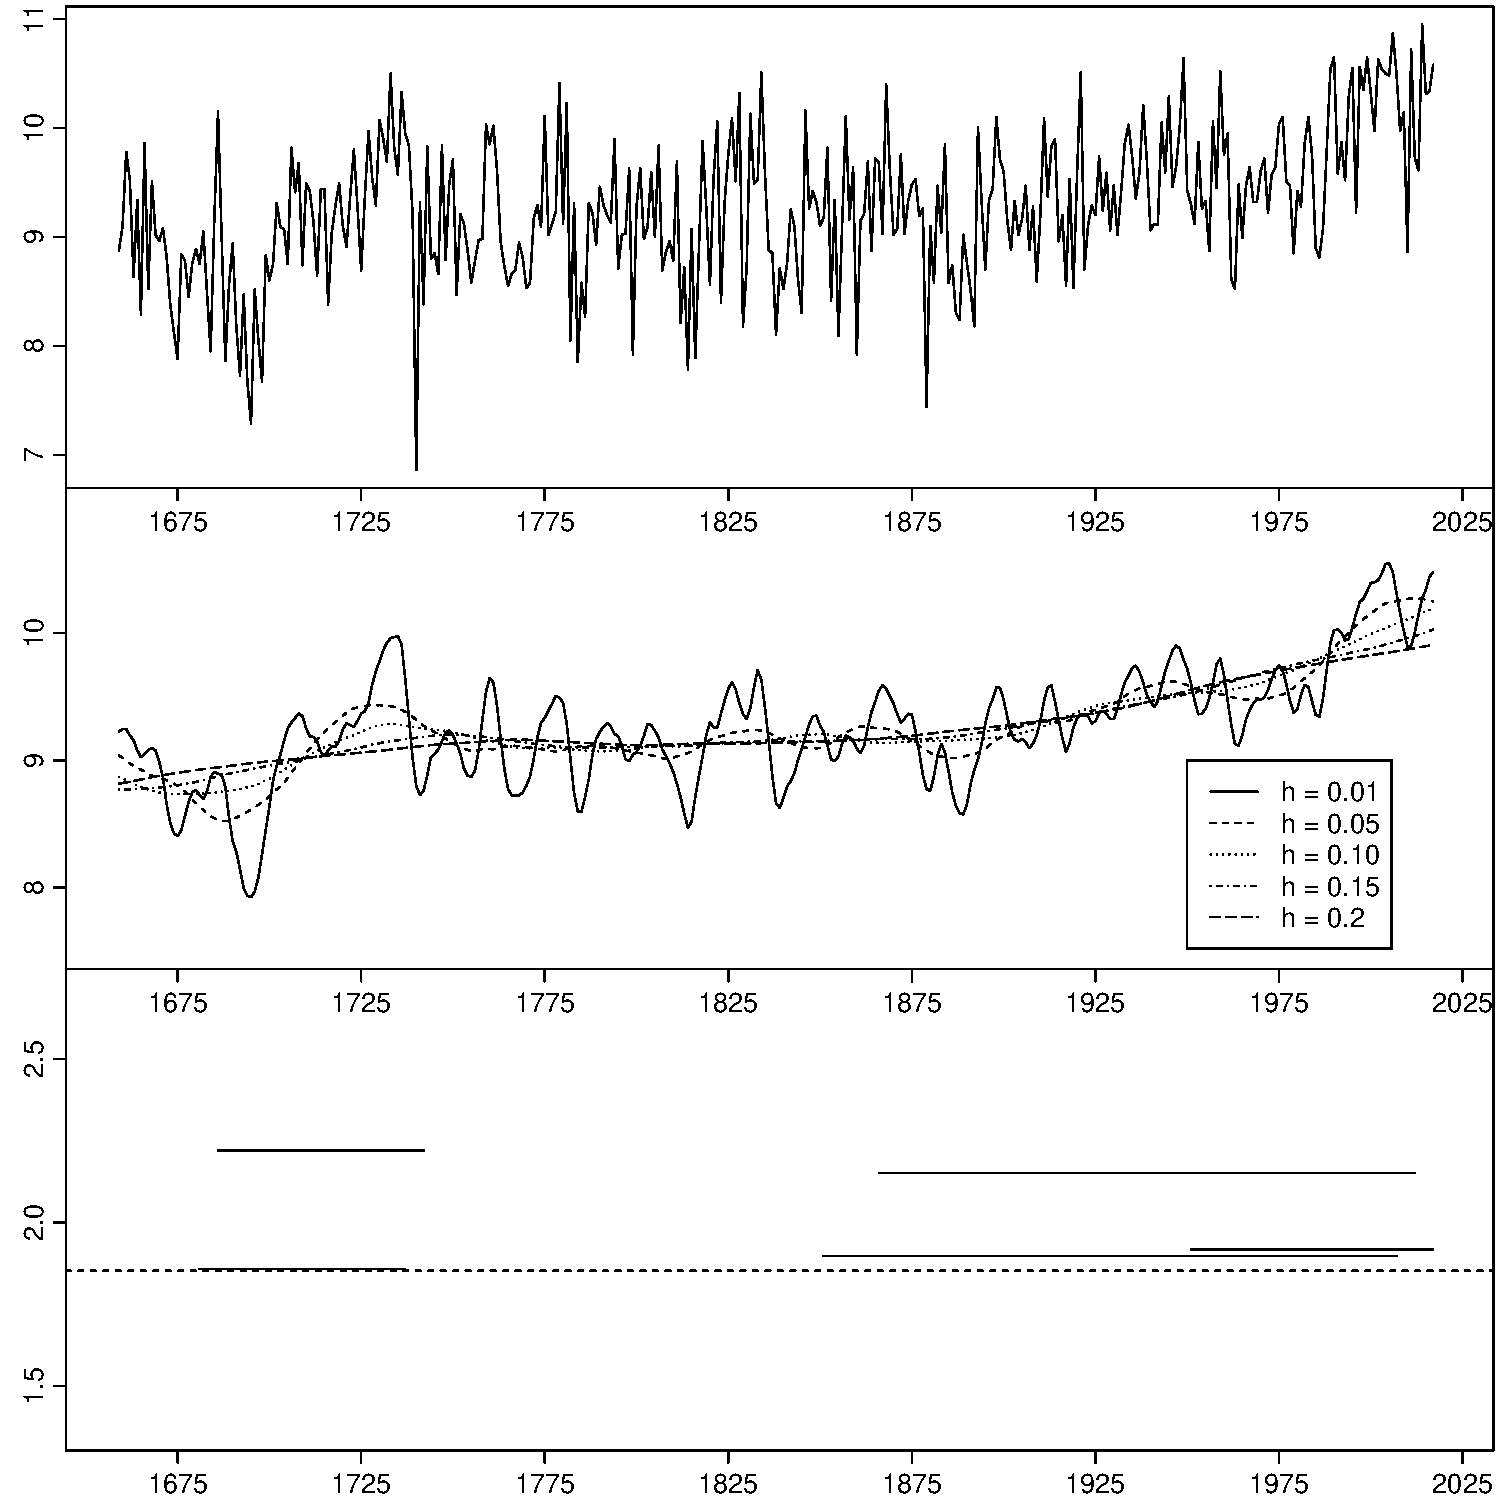
\includegraphics[width=0.8\textwidth]{Plots/threegraphics_testing_constant_method_ll.pdf}
\caption{Summary of the application results from Section \ref{subsec-data-1}. The upper panel shows the Central England mean temperature time series. The middle panel depicts local linear kernel estimates of the time trend for a number of different bandwidths $h$. The lower panel presents the minimal intervals in the set $\Pi_T^+$ produced by the multiscale test. These are $[1681,1737]$, $[1686,1742]$, $[1851,2007]$, $[1866,2012]$ and $[1881,2017]$.}\label{plot-results-app1}
\end{figure}


Our multiscale test provides this kind of information, which is summarized in the lower panel of Figure \ref{plot-results-app1}. The plot depicts the minimal intervals contained in the set $\Pi_T^+$ which is defined in Section \ref{subsec-test-shape-theo}. The set of intervals $\Pi_T^-$ is empty in the present case. The height at which a minimal interval $I_{u,h} = [u-h,u+h] \in \Pi_t^+$ is plotted indicates the value of the corresponding (additively corrected) test statistic $\widehat{\psi}^\prime_T(u,h) / \hat{\sigma} - \lambda(h)$. The dashed line specifies the critical value $q_T^\prime(\alpha)$, where $\alpha = 0.05$ as already mentioned above. According to Proposition \ref{prop-test-shape-2}, we can make the following simultaneous confidence statement about the collection of minimal intervals in $\Pi_T^+$. We can claim, with confidence of about $95\%$, that the trend function $m$ has some increase on each minimal interval. More specifically, we can claim with this confidence that there has been some upward movement in the trend both in the period from around $1680$ to $1740$ and in the period from around $1880$ onwards. Hence, our test in particular provides evidence that there has been some warming trend in the period over the last $150$ years or so. On the other hand, as the set $\Pi_T^-$ is empty, there is no evidence of any downward movement of the trend.  


\subsection{Analysis of UK weather station data}\label{subsec-data-2} 


\begin{figure}[t]
\centering
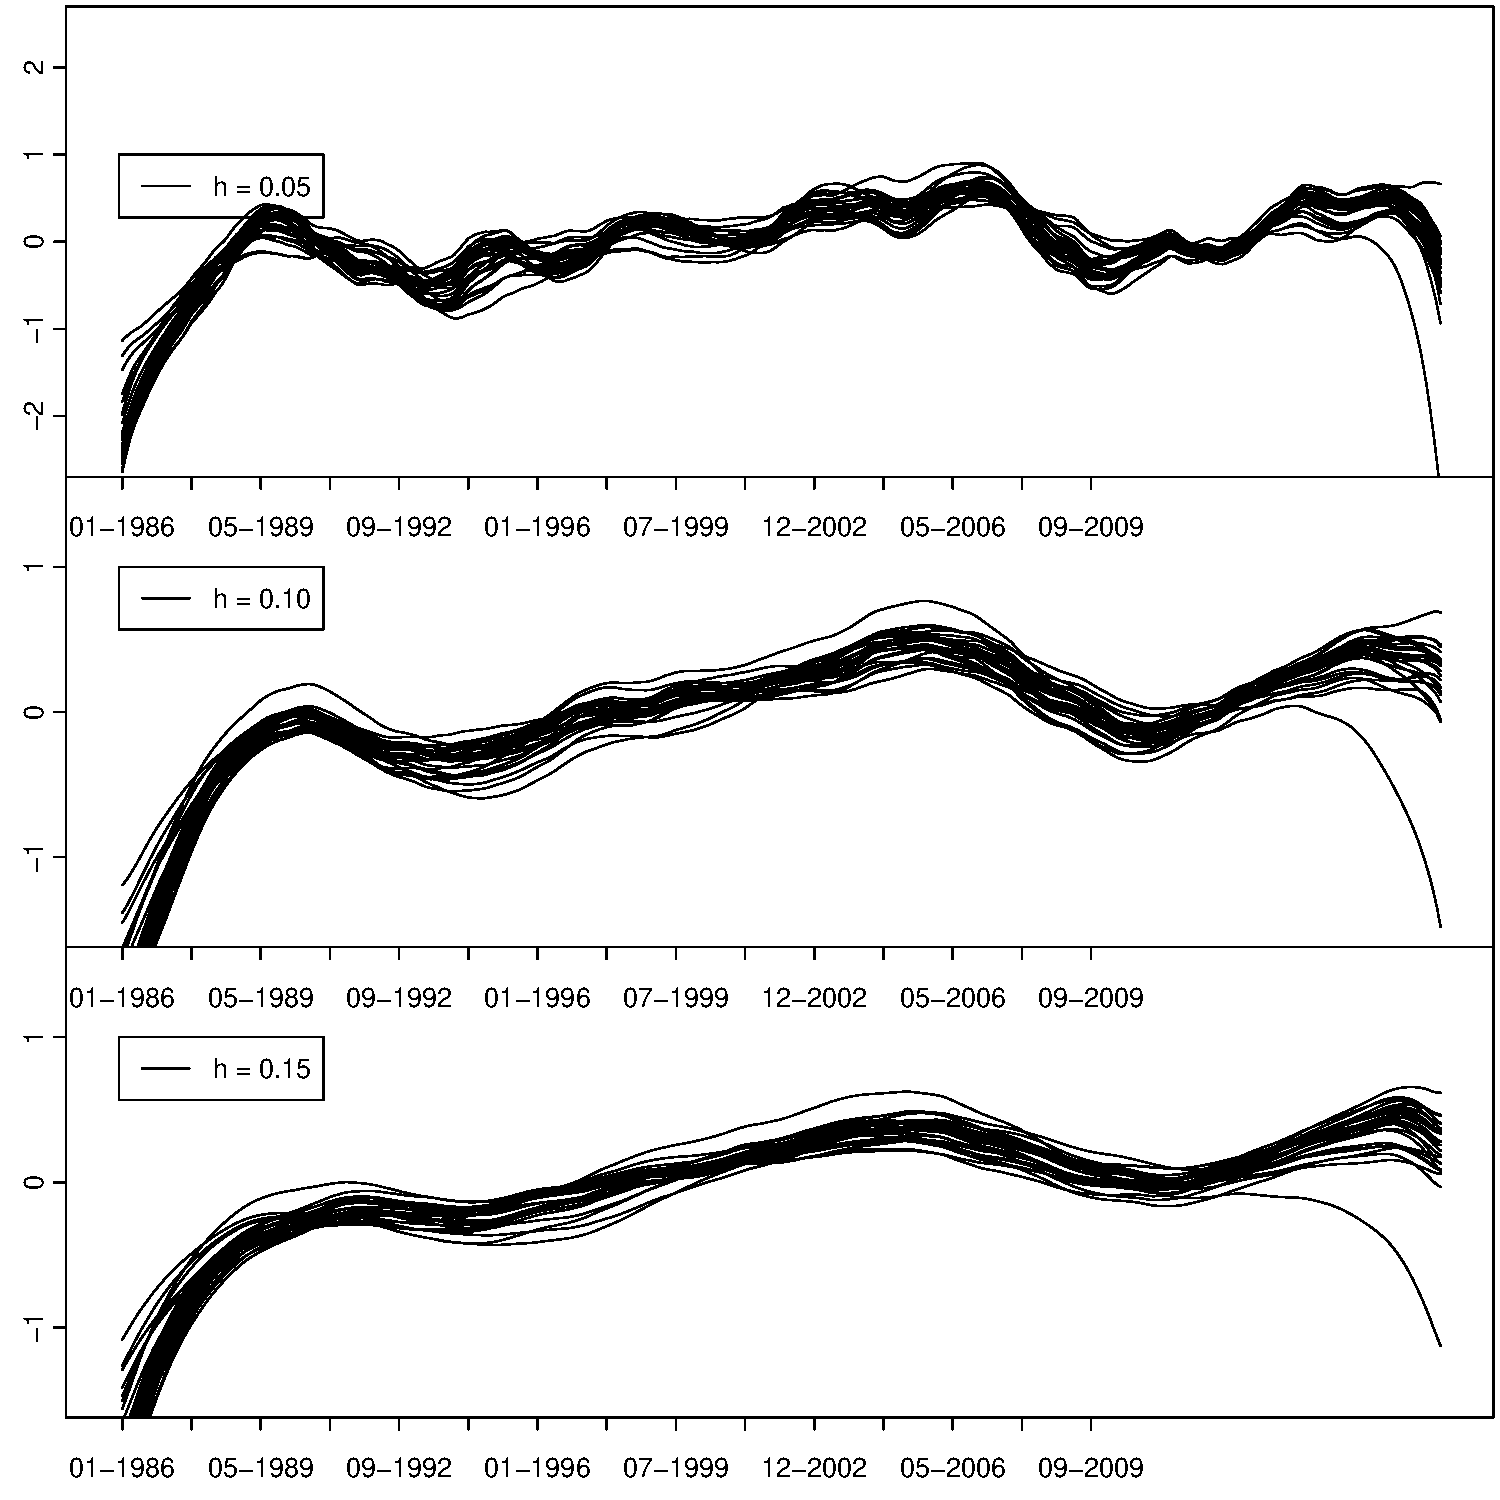
\includegraphics[width=0.8\textwidth]{Plots/stations_data.pdf}
\vspace{0.2cm}
\caption{Local linear kernel estimates of the $n=25$ time trends from the application of Section \ref{subsec-data-2}. Each panel shows the estimates for a different bandwidth $h$.}\label{plot-results-app2}
\end{figure}


To illustrate our test method from Section \ref{sec-test-equality}, we examine a dataset of monthly mean temperatures from $34$ different UK weather stations. As before, the data is publicly available on the webpage of the UK Met Office. We use a subset of $25$ stations for which data is available over the time span from $1986$ to $2017$. We thus observe a time series $\mathcal{Y}_i = \{Y_{it}: 1 \le t \le T \}$ of length $T = 396$ for each station $i \in \{1,\ldots,25\}$. The time series $\mathcal{Y}_i$ is assumed to follow the model 
\begin{equation}\label{model2-app}
Y_{it} = \alpha_i(t) + m_i\Big(\frac{t}{T}\Big) + \varepsilon_{it}, 
\end{equation}
where $m_i$ is an unknown nonparametric time trend and $\alpha_i(t)$ is a month-specific intercept which captures the seasonality pattern in the data. We suppose that $\alpha_i(t) = \alpha(t + 12 \ell)$ for any integer $\ell$, that is, we have a different intercept $\alpha_i(k)$ for each month $k = 1,\ldots,12$. The test method and the underlying theory from Section \ref{sec-test-equality} can be easily adapted to model \eqref{model2-app}, which is a slight extension of model \eqref{model2}. The details are provided below. As in Section \ref{subsec-data-1}, the error process $\mathcal{E}_i = \{ \varepsilon_{it}: 1 \le t \le T \}$ is assumed to have the AR(1) structure $\varepsilon_{it} = a_i \varepsilon_{i,t-1} + \eta_{it}$ for each $i$, where $\eta_{it}$ are i.i.d.\ innovations with mean zero.  


To illustrate our test method from Section \ref{sec-test-equality}, we examine a dataset of monthly mean temperatures from $34$ different UK weather stations. The data are publicly available on the webpage of the UK Met Office. We use a subset of $25$ stations for which data are available over the time span from $1986$ to $2017$. We thus observe a time series $\mathcal{Y}_i = \{Y_{it}: 1 \le t \le T \}$ of length $T = 396$ for each station $i \in \{1,\ldots,25\}$. The time series $\mathcal{Y}_i$ is assumed to follow the model 
\begin{equation}\label{model2-app}
Y_{it} = \alpha_i(t) + m_i\Big(\frac{t}{T}\Big) + \varepsilon_{it}, 
\end{equation}
where $m_i$ is an unknown nonparametric time trend and $\alpha_i(t)$ is a month-specific intercept which captures the seasonality pattern in the data. We suppose that $\alpha_i(t) = \alpha(t + 12 \ell)$ for any integer $\ell$, that is, we have a different intercept $\alpha_i(k)$ for each month $k = 1,\ldots,12$. The test method and the underlying theory from Section \ref{sec-test-equality} can be easily adapted to model \eqref{model2-app}, which is a slight extension of model \eqref{model2}. The details are provided below. As in Section \ref{subsec-data-1}, the error process $\mathcal{E}_i = \{ \varepsilon_{it}: 1 \le t \le T \}$ is assumed to have the AR(1) structure $\varepsilon_{it} = a_i \varepsilon_{i,t-1} + \eta_{it}$ for each $i$, where $\eta_{it}$ are i.i.d.\ innovations with mean zero.  


We aim to test whether the time trend $m_i$ is the same at each of the $25$ weather stations. In other words, we want to test the null hypothesis $H_0: m_1 = \ldots = m_n$ with $n = 25$ in model \eqref{model2-app}. To do so, we apply the multiscale test from Section \ref{sec-test-equality} with two minor modifications: (i) We define $\widehat{Y}_{it} = Y_{it} - \widehat{\alpha}_i(t)$, where $\widehat{\alpha}_i(t)$ is an estimator of $\alpha_i(t)$. In particular, we set $\widehat{\alpha}_i(k) = T_k^{-1} \sum_{t = 1}^T \ind_k(t) Y_{it}$, where $\ind_k(t) = \ind(t = k + \lfloor (t-1)/12 \rfloor \cdot 12)$ and $T_k = \sum_{t=1}^T \ind_k(t)$. (ii) We define the Gaussian statistic $\Phi_{n,T}$ as in Section \ref{subsec-test-equality-test} with $\phi_{ij,T}(u,h) = \sum_{t=1}^T w_{t,T}(u,h) \{ \widehat{\sigma}_i (Z_{it} - \bar{Z}_i(t)) - \widehat{\sigma}_j (Z_{jt} - \bar{Z}_j(t))\}$, where $\bar{Z}_i(t) = \sum_{k=1}^{12} 1_k(t) \{ T_k^{-1} \sum_{s = 1}^T \ind_k(s) Z_{is} \}$. Apart from these two modifications, the multiscale test is constructed exactly as described in Section \ref{sec-test-equality}. We implement the test in the same way as in the simulations of Section \ref{sec-sim}. 


We are now ready to apply the test procedure to the data. Figure \ref{plot-results-app2} depicts the local linear estimates of the trend functions $m_i$ for the $n=25$ different stations. Each panel corresponds to a different bandwidth $h$. As can be seen, for a given bandwidth $h$, the fits look very similar to each other. Visual inspection thus suggests that there are no strong differences between the time trends $m_i$. Our test confirms this impression. It does not reject the null hypothesis at the most common levels $\alpha = 0.01, 0.05, 0.1$. Hence, the test does not provide any evidence for a violation of the null. %our test provides evidence that there is no difference between the trends from the $n=25$ weather stations during the observation period from $1986$ to $2017$.

